%% ------------------------------------------------------------------------- %%
\newcommand{\splits}{cortes }
\newcommand{\splitt}{corte }
\newcommand{\concatenations}{concatenações }
\newcommand{\concatenation}{concatenação }
\newcommand{\str}{string}
\newcommand{\Str}{String}

\chapter{Florestas dinâmicas}
\label{cap:florestas}

O problema da floresta dinâmica consiste em manter uma coleção de árvores enraizadas disjuntas que são modificadas ao longo do tempo pela adição e remoção de arestas. De forma objetiva, queremos realizar às seguintes operações:

\begin{itemize}
    \item inicializa($n$): Cria $n$ árvores disjuntas, todas com apenas um vértice. Os vértices são numerados de $1$ até $n$.
    \item raiz($v$): Devolve a raiz da árvore que contém $v$.
    \item liga($u,v$): Combina as árvores contendo $u$ e $v$ pela adição da aresta $\{u,v\}$. Supõe que $u$ e $v$ estão em árvores diferentes.
    \item corta($u,v$): remove a aresta $\{u,v\}$. Supõe que a aresta $\{u,v\}$ existe.
\end{itemize}

Ao longo deste capítulo, denotamos por $n$ o parâmetro da operação inicializa, isto é, o número de vértices da floresta. Também denotamos por $m$ o número de operações raiz, liga e corta.

Uma maneira de resolver o problema é armazenar a floresta numa matriz de adjacência. Com essa representação, cada operação liga e corta consome tempo $O(1)$, mas a operação raiz consome tempo proporcional a profundidade do vértice, que é $O(n)$.

Ao representar as árvores de outra forma, reduziremos a complexidade da operação raiz para $O(\log n)$, pagando o preço de aumentar o consumo de tempo das operações de liga e corta também para $O(\log n)$.

\section{Sequências}
\label{sec:sequencia}
Uma \textbf{\str} é uma sequência finita de elementos. 

\section{Sequências de Euler}
\label{sec:sequencia-euler}

Definimos a \textbf{sequência de Euler} de uma árvore enraizada num vértice $r$ por ET($r$), onde ET é definido como:

\begin{algorithmic}[H]
\Function{ET}{$u$}
    \State acrescente \texttt{uu}
    \ForAll{$v$ vizinho de $u$}
        \State acrescente \texttt{uv}
        \If{$v$ não foi visitado}
            \State \Call{ET}{$v$}
        \EndIf
    \EndFor
\EndFunction
\end{algorithmic}

Ao aplicar o procedimento no vértice \texttt{A} da figura \ref{fig:euler-exemplo}, vemos que a sequência eureliana é $\mathtt{AA\,AB\,BB\,BE\,EE\,EB\,BA\,AC\,CC\,CF\,FF\,FC\,CG\,GG\,GC\,CA\,AD\,DD\,DA}$. Note que a raiz da árvore sempre será o primeiro elemento da sequência.

\begin{figure}[H]
    \caption{Árvore enraizada no vértice A}
    \label{fig:euler-exemplo}
        \centering
        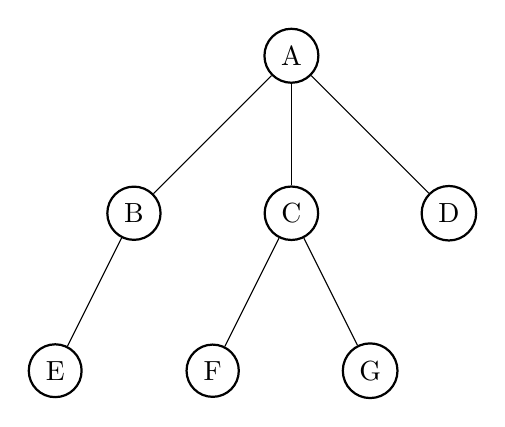
\begin{tikzpicture}[every node/.style={circle,thick,draw}]
            \node (A) at (0,0) {A};
            \node (B) at (-2,-2) {B};
            \node (C) at (0,-2) {C};
            \node (D) at (2,-2) {D};
            \node (E) at (-3,-4) {E};
            \node (F) at (-1,-4) {F};
            \node (G) at (1,-4) {G};
            \path [-] (A) edge (B);
            \path [-] (A) edge (C);
            \path [-] (A) edge (D);
            \path [-] (B) edge (E);
            \path [-] (C) edge (F);
            \path [-] (C) edge (G);
        \end{tikzpicture}
\end{figure}

A sequência eureliana de uma árvore é na verdade o circuito eureliano do grafo gerado pela duplicação de suas arestas e inclusão de laços em todos seus vértices (veja a figura \ref{fig:euler-exemplo-duplicado}).

\begin{figure}[H]
    \caption{Grafo induzido pela duplicação e adição de laços na árvore da figura \ref{fig:euler-exemplo}}
    \label{fig:euler-exemplo-duplicado}
    \centering
        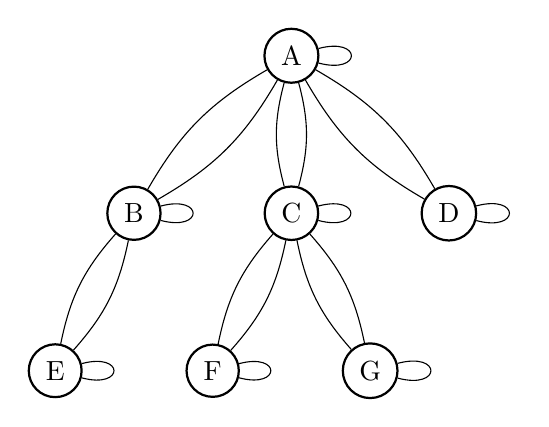
\begin{tikzpicture}[every node/.style={circle,thick,draw}, every loop/.style={}]
            \node (A) at (0,0) {A};
            \node (B) at (-2,-2) {B};
            \node (C) at (0,-2) {C};
            \node (D) at (2,-2) {D};
            \node (E) at (-3,-4) {E};
            \node (F) at (-1,-4) {F};
            \node (G) at (1,-4) {G};
            \path [-] (A) edge[bend right=15] (B);
            \path [-] (A) edge[bend left=15] (B);
            \path [-] (A) edge[bend right=15] (C);
            \path [-] (A) edge[bend left=15] (C);
            \path [-] (A) edge[bend right=15] (D);
            \path [-] (A) edge[bend left=15] (D);
            \path [-] (B) edge[bend right=15] (E);
            \path [-] (B) edge[bend left=15] (E);
            \path [-] (C) edge[bend right=15] (F);
            \path [-] (C) edge[bend left=15] (F);
            \path [-] (C) edge[bend right=15] (G);
            \path [-] (C) edge[bend left=15] (G);
            \path [-] (A) edge[loop right] (A);
            \path [-] (B) edge[loop right] (B);
            \path [-] (C) edge[loop right] (C);
            \path [-] (D) edge[loop right] (D);
            \path [-] (E) edge[loop right] (E);
            \path [-] (F) edge[loop right] (F);
            \path [-] (G) edge[loop right] (G);
        \end{tikzpicture}
\end{figure}

Note que uma sequência eureliana define unicamente uma árvore, já que contém todos seus vértices e arestas. Por esse motivo, podemos representar árvores por sequências eurelianas. Essa representação é enxuta e nos permite realizar as operações de liga, corta e raiz de forma simples, como veremos adiante.

\begin{prop}
    \label{prop:seq-3n}
    Uma sequência eureliana de uma árvore com $n$ vértices tem tamanho $3n-2$.
\end{prop}

\begin{proof}
Seja $T$ uma árvore com $n$ vértices. Cada aresta de $T$ aparece duas vezes na sequência e cada vértice aparece uma vez na forma de um laço, portanto temos ${2(n-1) + n = 3n-2}$ elementos.
\end{proof}

Vamos analisar o que acontece com a sequência eureliana da árvore da figura \ref{fig:euler-exemplo} quando removemos a aresta $AC$. A figura \ref{fig:euler-exemplo-remove-ac} ilustra o resultado da operação.

\begin{figure}[H]
    \caption{Resultado da remoção da aresta $AC$.}
    \label{fig:euler-exemplo-remove-ac}
        \centering
        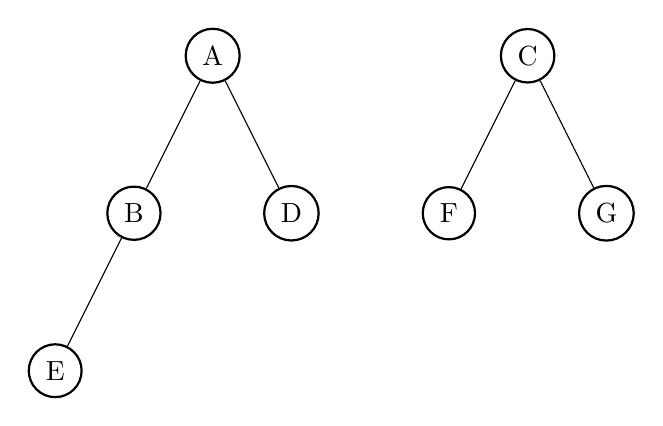
\begin{tikzpicture}[every node/.style={circle,thick,draw}]
            \node (A) at (-1,0) {A};
            \node (B) at (-2,-2) {B};
            \node (D) at (0,-2) {D};
            \node (E) at (-3,-4) {E};
            
            \node (C) at (3,0) {C};
            \node (F) at (2,-2) {F};
            \node (G) at (4,-2) {G};
            
            \path [-] (A) edge (B);
            \path [-] (A) edge (D);
            \path [-] (B) edge (E);
            
            \path [-] (C) edge (F);
            \path [-] (C) edge (G);
        \end{tikzpicture}
\end{figure}

Se tomarmos o vértice $C$ como raiz da nova árvore que contém $C$, a sequência eureliana dessa árvore é \eqref{bla} $\mathtt{CC}\,\mathtt{CF}\,\mathtt{FF}\,\mathtt{FC}\,\mathtt{CG}\,\mathtt{GG}\,\mathtt{GC}$. Mantendo o vértice $A$ como raiz da outra árvore, temos a sequência eureliana $\mathtt{AA\,AB\,BB\,BE\,EE\,EB\,BA\,AD\,DD\,DA}$. Nesse caso, vemos que a sequência eureliana da árvore que contém $C$ é uma subsequência contínua da sequência eureliana da árvore antes da remoção da aresta $AC$. Similarmente, a sequência eureliana da árvore que contém $A$ é uma concatenação de duas subsequências contínuas da sequência eureliana original.

\begin{align}
 \rightarrow & \mathtt{AA\,AB\,BB\,BE\,EE\,EB\,BA\,\underline{AC}\,CC\,CF\,FF\,FC\,CG\,GG\,GC\,\underline{CA}\,AD\,DD\,DA} \label{bla}\\
\rightarrow & \mathtt{AA\,AB\,BB\,BE\,EE\,EB\,BA\,\phantom{AC\,}CC\,CF\,FF\,FC\,CG\,GG\,GC\,\phantom{CA\,}AD\,DD\,DA} \nonumber
\end{align}


\begin{prop}
Sejam $T$ uma árvore e $S$ uma sequência eureliana de $T$. Para toda aresta $e$ de $T$, é possível obter uma sequência eureliana das duas árvores de $T - e$ com quatro \splits e uma \concatenation.
\end{prop}
\begin{proof}
Seja $e = uv$ uma aresta de $T$. Suponha sem perda de generalidade que $\mathtt{uv}$ ocorre antes de $\mathtt{vu}$ em $S$. Logo, $S$ é da forma $S_1\,\mathtt{uv}\,S_v\,\mathtt{vu}\,S_2$, onde $S_v$ é a sequência eureliana da árvore de $T-e$ enraizada em $v$. Com quatro \splits extraímos $S_v$ e removemos $\mathtt{uv}$ e $\mathtt{vu}$. Uma \concatenation $S_1S_2$ nos dá a sequência eureliana da nova árvore enraizada em $u$.
\end{proof}

%\begin{prop}
%Sejam $T$ uma árvore enraizada e $S$ uma sequência eureliana de $T$. Para todo vértice $v$ de $T$, é possível obter uma sequência eureliana de $T$ que começa e termina em $v$ com um \split e uma \concatenation.
%\end{prop}
%Seja $v$ um vértice de $T$. Note que $S$ é da forma $S_1\,\mathtt{vv}\,S_2$, onde o primeiro vértice de $S_1$ é o último vértice de $S_2$. Logo, a sequência $vvS_2S_1$ é uma sequência eureliana de $T$, que começa e termina em $v$.

Continuando com nosso exemplo, vamos analisar o que acontece quando adicionamos a aresta $DG$ na floresta da figura \ref{fig:euler-exemplo-remove-ac}. O resultado da operação é ilustrado na figura \ref{fig:euler-exemplo-adiciona-dg}.

\begin{figure}[H]
        \centering
        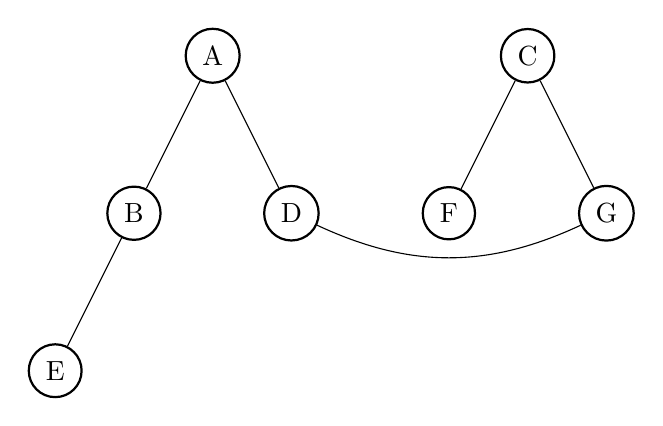
\begin{tikzpicture}[every node/.style={circle,thick,draw}]
            \node (A) at (-1,0) {A};
            \node (B) at (-2,-2) {B};
            \node (D) at (0,-2) {D};
            \node (E) at (-3,-4) {E};
            
            \node (C) at (3,0) {C};
            \node (F) at (2,-2) {F};
            \node (G) at (4,-2) {G};
            
            \path [-] (A) edge (B);
            \path [-] (A) edge (D);
            \path [-] (B) edge (E);
            
            \path [-] (C) edge (F);
            \path [-] (C) edge (G);
            
            \path [-] (D) edge[bend right=25] (G);
        \end{tikzpicture}
        \caption{Resultado da adição da aresta $DG$.}
        \label{fig:euler-exemplo-adiciona-dg}
\end{figure}

Há algo estranho na figura. Ainda que ela represente corretamente a nova árvore, vamos dar um passo atrás e re-enraizar as árvores nos vértices $D$ e $G$, como ilustrado na figura \ref{fig:euler-exemplo-re-enraiza}.

\begin{figure}[H]
    \caption{Árvores re-enraizadas nos vértices $D$ e $G$.}
    \label{fig:euler-exemplo-re-enraiza}
        \centering
        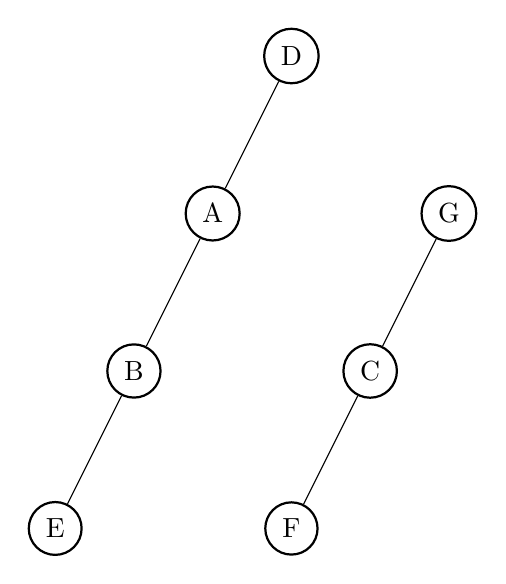
\begin{tikzpicture}[every node/.style={circle,thick,draw}]
            \node (A) at (-3,0) {A};
            \node (B) at (-4,-2) {B};
            \node (D) at (-2,2) {D};
            \node (E) at (-5,-4) {E};
            
            \node (C) at (-1,-2) {C};
            \node (F) at (-2,-4) {F};
            \node (G) at (0,0) {G};
            
            \path [-] (A) edge (B);
            \path [-] (A) edge (D);
            \path [-] (B) edge (E);
            
            \path [-] (C) edge (F);
            \path [-] (C) edge (G);
        \end{tikzpicture}
\end{figure}

Note que ao re-enraizar uma árvore, sua sequência eureliana muda. Nesse caso, as novas sequências são $\mathtt{DD\,DA\,AA\,AB\,BB\,BE\,EE\,EB\,BA\,AD}$ e $\mathtt{GG\,GC\,CC\,CF\,FF\,FC\,CG}$. Ambas são rotações das sequências originais. Ao se adicionar a aresta $DG$ nessa nova configuração, a nova sequência é $\mathtt{DD\,DA\,AA\,AB\,BB\,BE\,EE\,EB\,BA\,AD\,DG\,GG\,GC\,CC\,CF\,FF\,FC\,CG\,GD}$, uma simples concatenação das sequências originais e da nova aresta.  

\begin{prop}
Sejam $T_1$ e $T_2$ duas árvores disjuntas e $S$ e $R$ sequências eurelianas de $T_1$ e $T_2$, respectivamente. Para todo vértice $u \in T_1$ e $v \in T_2$, é possível obter a sequência eureliana de $(T_1 \cup T_2) + uv$ com quatro \concatenations e um \splitt. 
\end{prop}
\begin{proof}
Sejam $u$ e $v$ vértices de $T_1$ e $T_2$, respectivamente. Note que $S = S_1\,\mathtt{uu}\,S_2$ e $R = R_1\,\mathtt{vv}\,R_2$. Definimos $S' := \mathtt{uu}\,S_2S_1$ e $R' :=\mathtt{vv}\, R_2R_1$. Logo, $S'\,\mathtt{uv}\,R'\,\mathtt{vu}$ é uma sequência eureliana de $(T_1 \cup T_2) + uv$ enraizada em $u$.
\end{proof}

As proposições apresentadas reduzem o problema da floresta dinâmica para o problema de concatenar e fatiar sequências. No capítulo \ref{cap:sequencias} apresentamos uma maneira eficiente de se representar e realizar as operações em sequência.




